\section{Ciência e colaboração}

\subsection{Reprodutibilidade}

Enquanto pesquisadores publicam artigos descrevendo e divulgando seus
resultados, é raro que façam o mesmo com toda a produção gerada durante a
pesquisa. A maioria dos componentes necessários para a reprodução dos
resultados de uma pesquisa -- por exemplo, códigos fonte e dados -- usualmente
permanecem não publicados. Esse problema fere um dos fundamentos
da ciência de que novas descobertas sejam reproduzidas antes de serem
consideradas parte da base de conhecimento \cite{Stodden2009}.

%Nesse sentido, \citeonline{Prlic2012} enfatizam que disponibilizar o código
%criado durante pesquisas não apenas aumenta o impacto como também se torna
%essencial para outros reproduzirem os resultados encontrados, citam ainda que
%manutenabilidade e disponibilidade do software após a publicação é o maior
%problema enfrentado pelos pesquisadores que desenvolvem tais softwares.
%
%A replicação desses estudos empíricos pode, e deve, ser realizado, de modo a
%averiguar a validade e aumentar o nível de confiança em seus resultados,
%replicação costuma ser citado como um importante meio para validar estudos
%empíricos e assim aumentar o nível de confiança em seus resultados
%\cite{Almqvist2006}. A reprodução dos resultados de pesquisas aumenta o impacto
%social das pesquisas e gera economia de tempo e dinheiro para os pesquisadores
%e para as instituições \cite{Nesta2010}.

Apesar da preocupação com a reprodutibilidade dos resultados de pesquisas de
forma independente \cite{Stodden2009} e aberta, esta área tem recebido ainda
pouca atenção da comunidade de pesquisa \cite{Nancy2015, Grand2010Open}. Em um
estudo recente, com 88 papers do MSR entre 2004-2011, evidenticou-se que apenas
62\% são replicaveis ou parcialmente replicaveis e que apenas 20\% dos estudos
disponibilizam suas ferramentas \cite{amann2015software}. Um estudo anterior
com 171 papers do MSR evidenciam que, entre outros problemas, a maioria não
disponibilizam publicamente as ferramentas e scripts, mesmo quando os autores
explicitamente afirmam que construíram algum \cite{robles2010replicating},
apenas 2 entre 154 estudos experimentais avaliados fornecem os dados e as
ferramentas necessárias para replicação e futuras pesquisas
\cite{barr2010shoulders}.

Reprodutibilidade ({\it reproducibility}) é a habilidade de replicar um experimento
ou estudo em sua totalidade a fim de confirmar suas hipóteses, seja pelo
autor ou por pesquisadores independentes. Esse conceito é um ponto
central do método científico e continua a receber bastante atenção ainda hoje,
como pode ser verificado em estudos recentes.

\citeonline{Stodden2009} preocupada com as barreiras legais para
disponibilidade de artefatos de pesquisa propõe o framework ``{\it Reproducible
Research Standard (RRS)}'', onde sugere formas de usar o licenciamento e as leis
de copyright da melhor forma para manter disponíveis os produtos gerados
durante pesquisas e assim viabilizar reprodutibilidade. \citeonline{Vitek2011}
em um estudo sobre reprodutibilidade e rigor científico destacam a importancia
de se disponibilizar qualquer material suplementar gerado durante uma pesquisa
de modo a possibilitar revisores verificarem e replicarem experimentos. Em
2012, um workshop intitulado ``{\it Reproducible Research: Tools and Strategies for
Scientific Computing}'' \cite{Stodden2012} discutiu, especificamente, iniciativas
e ferramentas voltadas a apoiar pesquisas reprodutíveis.
\citeonline{Krishnamurthi2015}, em um estudo sobre repetibilidade, chamam
atenção para o papel central que os artefatos de software possuem em pesquisas
de ciência da computação e questionam: "Onde está o software nas pesquisas
sobre linguagem de programação?". \citeonline{Stodden2015} demonstram o
projeto "ResearchCompendia.org", uma infraestrtura para reprodutibilidade e
colaboração em ciência computacional. Além destes e tantos outros estudos em
\cite{GithubReproducibilityGuide} é possível acessar um guia sobre como
desenvolver pesquisas cientíticas de forma que promovam a reprodutibilidade.

Apesar do termo reprodutibilidade ser relativamente concensual entre as várias
áreas da ciência, existem alguns termos relacionados com uma certa diferença
de significado, diante disto, e preocupado em criar uma linguagem comum entre
os pesquisadores, \citeonline{Feitelson2015} propôs as seguintes definições:

\begin{description}

  \item[Repetição (repetition)]
  Refazer exatamente o que outra pessoa fez usando os artefatos originais.

  \item[Replicação (replication)]
  Replicar com precisão exatamente o que outra pessoa fez, recriando os
  artefatos.

  \item[Variação (variation)]
  Repetir ou replicar exatamente o que a outra pessoa fez, mas com alguma
  modificação controlada nos parâmetros.

  \item[Reprodução (reproduction)]
  Recriar o espírito do que outra pessoa fez, usando seus próprios artefatos.

  \item[Corroboração (corroboration)]
  Obter os mesmos resultados de outra pessoa, usando outros meios e
  procedimentos experimentais.

\end{description}

É conhecido que a ciência precisa de reprodutibilidade e corroboração para
realmente fazer progressos, mas a prática de forma abrangente ainda é um
obstáculo. Diante disso \citeonline{Peng2011} sugere adotar soluções
intermediárias, repetição, replicação, variação, e desta forma já teríamos uma
grande melhoria sobre a situação atual onde muitos estudos em engenharia de
software sofrem de dificuldades de repetição \cite{Tang2016} e,
consequentemente, poucos estudos replicando pesquisas da área são encontrados
\cite{da2011replication}.

Mesmo sabendo que todo artefato tem impacto na reprodutibilidade
\cite{gonzalez2012reproducibility}, uma barreira comum para tal prática, e
consequentemente para repetição, replicação e variação é a indisponibilidade do
código fonte. Toda pesquisa que possua qualquer processo computadorizado deve
publicar seus códigos, eles precisam estar disponíveis, mesmo que os dados
correspondentes não estejam, o código deve estar. De acordo com o espectro de
reprodutibilidade (Figura \ref{reproducibility-spectrum}), a disponibilidade de
código é o requisito mínimo e é o primeiro passo para possibilitar validação e
confirmação dos resultados.

\begin{figure}[h]
  \center
  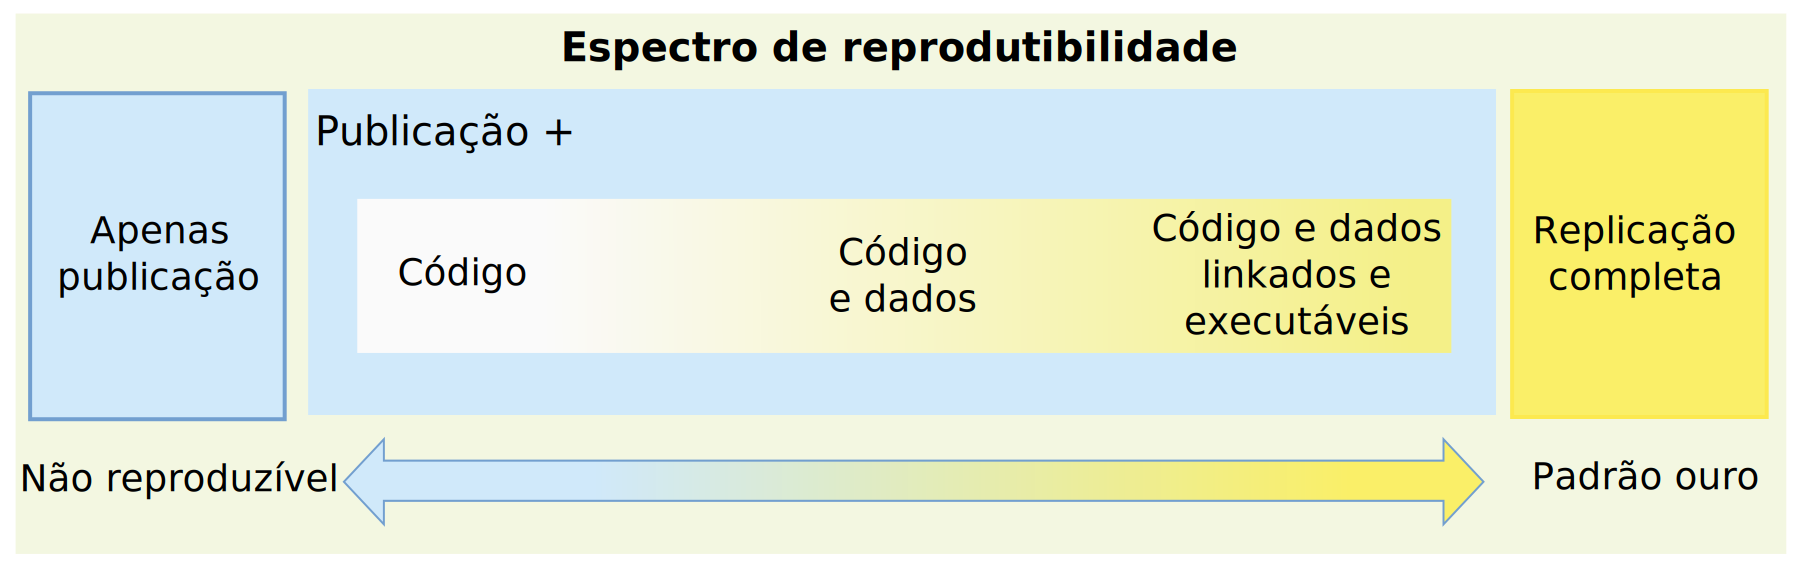
\includegraphics[scale=0.35]{imagens/reproducibility-spectrum-ptbr.png}
  \caption{Espectro de reprodutibilidade \cite{Peng2011}}
  \label{reproducibility-spectrum}
\end{figure}

Apesar das pesquisas reproduzíveis ({\it RR - Reproducible Research}) não
resolverem todos os problemas de validade experimental dos estudos em
engenharia de software, elas ao menos garantem que dados e métodos de análise
estejam disponíveis para inspeção e que os resultados possam ser derivados,
facilitando revisão logo que a publicação acontece. Além disso, é um recurso
valoroso para pesquisadores iniciantes, pesquisas reproduzíveis melhoram o
impacto do próprio estudo, por exemplo, artigos de computação que não
disponibilizam pubicamente dados e códigos possuem menos chances de serem
citados \cite{madeyski2017would}.

\subsection{Ciência aberta}

Ciência Aberta é um movimento que tem por objetivo tornar a pesquisa
científica, seus dados e sua disseminação acessíveis à todos os interessados,
sejam amadores ou profissionais \cite{WikipediaOpenScience}. Sua principal
motivação está em possibilitar a reprodução dos resultados de pesquisas e em
garantir transparência das metodologias utilizadas, isto aumenta o impacto
social das pesquisas e gera economia de tempo e dinheiro para os pesquisadores
e para as instituições \cite{Nesta2010}.

Este movimento é guiado por princípios básicos de transparência, acessibilidade
e reusabilidade universais, disseminadas via ferramentas online, ele é dividido
em quatro grandes áreas: (1) Open Access, (2) Open Data, (3) Open Source e (4)
Open Reproducible Research. Dentre elas destaca-se a Open Reproducible Research
por preocupar-se com a reprodutibilidade dos resultados de pesquisas de forma
independente \cite{Stodden2009} e aberta, no entanto, esta área tem recebido
ainda pouca atenção da comunidade de pesquisa \cite{Nancy2015}
\cite{Grand2010Open} apesar do aumento geral do interesse pelas práticas da
Ciência Aberta \cite{Grand2010}.

%Over the past fifteen years the scholarly communications agenda
%has progressed gradually. Currently we are experiencing a strong
%tendency among all research stakeholders to engage with the
%practice of OS. Lately, research funders require the sharing not
%only of the research results they have funded, but also of the
%procedures and data that are being generated during the research
%conduct. Researchers, on the other side, are keen on observing
%their research results being used for the improvement of the
%society and are forced by their funders to demonstrate the impact
%of their research. At the same time, higher academic institutions
%aim to join the OS agenda as well, since they see the opportunity
%of great economic benefits and savings. While OS is the possible
%answer to all these factors, the stakeholders’ inability to
%understand the requirements for the application of OS can be a
%suspensory factor for the OS implementation and evolution.
%The aim of the FOSTER project is to advance the stakeholders'
%knowledge on the usefulness of OS and explain the technicalities,
%strategies and best practices using which OS can be applied. As an
%attempt to educate the largest number of researchers possible,
%FOSTER has created an e-leanring portal, which contains quality
%assured information relating to the topic and it is open to everyone
%in the world. The platform contains two types of information:
%learning material and online courses. The classification of these
%two types is supported by an OS taxonomy, where related terms
%are applied both in the portal's material and also in the courses.
%With the use of the taxonomy, users are in the position to
%understand the OS domain and the concepts around it.
%The main goal of the FOSTER project, which is mainly achieved
%through the portal functionalities, is not only to educate the
%research stakeholders on OS, but also to build a community of
%researchers, librarians, software developers, funders and research
%administrators who are interested in OS in order to advance the
%way research is being conducted and shared. In addition, FOSTER
%attempts to provide tools to this community, such as re-usable
%content for training and a platform for blended learning and e-
%learning courses that the community could run. This OS
%advancement is essential for the research promotion and,
%consequently, for the benefit of the society as a whole
%\cite{Nancy2015}.
%
%Open Science may be practised both
%for philosophical and pragmatic reasons. As the
%resources produced by open projects are
%potentially accessible to public audiences, Open
%Science offers both a novel medium for public
%access and involvement in the process of science
%and an innovative method for real-time science
%communication. Does such direct access clear
%the stream of communication or muddy the
%waters with unfocussed, unclear and unvetted
%comment? This paper suggests that adopting an
%Open Science approach allows the capture of an
%authentic and clear record of research.
%However, researchers acknowledge this involves
%opening their work up to a different type of
%scrutiny \cite{Grand2010}.
%
%Open Science is an emerging approach to the conduct of science, technology and engineering
%projects, in which information about the whole of an ongoing investigation is made available
%on and through the Internet. Adopting an Open Science approach means the audience for the
%research can extend beyond the researchers involved to other researchers and to members of
%the public. Thus, Open Science has implications for engineering research, practice,
%publishing and public engagement with engineering. This paper reviews the history and
%evolution of the Open Science movement, includes some reflections on the related areas of
%Open Access, peer-review and public engagement with science and engineering and discusses
%data gathered from interviews. The analysis suggests that interviewees have concerns about
%issues such as precedence and protection of original work and the time needed to integrate
%open science practices into daily work. Successfully working in such collaborations is likely
%to require not only common practical tools but also the development of shared language and
%understanding between researchers and members of the public. Interviewees recognise the
%value of Open Science in collaborative research and its innovative facility to sustain direct
%public access to research outputs. It also has the potential to allow members of the public to
%make real practical contributions to research \cite{Grand2010Open}.
%
%This white paper was written as a contribution to the “Imagining
%Tomorrow’s University: Rethinking scholarship, education, and institu-
%tions for an open, networked era” workshop, a joint NIH/NSF-funded
%event held 8–9 March 2017 in Rosemont, IL. In this paper, I present an
%overview of what I consider open science, its importance, and how it
%plays a role in my research agenda. I also discuss challenges faced in
%pursuing research openness, and recommend changes to university
%leaders to address these barriers \cite{niemeyer2017open}.
%
%Open to All?  Case studies of openness in research
%Since the early 1990s, the open access movement has promoted the concept of openness in relation
%to scientific research. Focusing initially upon the records of science in the form of the text of articles
%in scholarly journals, interest has broadened in the last decade to include a much wider range of
%materials produced by researchers. At the same time, concepts of openness and access have also
%developed to include various kinds of use, by machines as well as humans.
%Academic bodies, including funders and groups of researchers, have set out statements in support
%of various levels of openness in research. Such statements often focus upon two key dimensions:
%what is made open, and how; and to whom is it made open, and under what conditions? This study
%set out to consider the practice of six research groups from a range of disciplines in order to better
%understand how principles of openness are translated into practice \cite{Nesta2010}.

\subsection{Ciberinfraestrutura}

A visão da ciberinfraestrutura, expressada no "Relatório Atkins" e instanciada
para o ecossistema de software científico na NSF chamada de Infraestrutura de
Software para Inovação Sustentada (NSF SI2),

Os softwares vem não apenas atuando no avanço da ciência, mas atuando com uma
eficiência crescente ao longo do tempo (Atkins 2003). A chave para isso é a
crença de que o software deve evoluir em direção a uma plataforma
compartilhada, com componentes que são reutilizados o mais amplamente possível,
já que os usuários finais e os produtores de componentes se agrupam em torno de
peças específicas de software.

a literatura sobre plataformas de software fora da ciencia tem chamado isso de
'coring' e 'tipping' (Gawer and Cusumano 2008),
onde uma comunidade descobre sua funcionalidade compartilhada e se agrupa
em pacotes que fornecem, levando ao uso eficiente de recursos através de
economias de escala.

coring também resulta em um aumento do uso sobreposto que facilita mais

Isto também resulta em um aumento do uso sobreposto que facilita mais
transparência na ciência, levando a uma maior qualidade e correctude (correctness), à medida
que mais olhos e esforços são direcionados para os mesmos códigos que são
sustentados e evoluem em longos períodos de utilidade científica.

coring em direção às plataformas pode ser contrastado com o seu oposto, muitas
vezes percebido por informantes: churn caótico disfuncional, com muitos
projetos com poucos usuários, cada um tendo vidas curtas que terminam com o
financiamento de concessão inicial, comunidades desconectadas e paralelas,
incompatibilidades teimosamente imutáveis e periódicas e tentativas
aparentemente não coordenadas de "reiniciar". Subjacente a isso é uma
preocupação que as oportunidades são perdidas e que o progresso da ciência é
abrandado (por exemplo, Stewart, Almes e Wheeler 2010).


%%%%%%%%%%%%%%%%%

O ecosistema de software acadêmico é um sistema que consome tempo, dinheiro e
atençao, e afeta a conduta e os resultados da ciência, tanto no geral, como em
campos específicos

chape para isto é acreditar que software deve evoluir para plataformas compartilhadas,
com componentes reusáveis tanto quanto possível, tanto para usuário final, quanto
para produtores de componentes (papel) agregando peças particulares de software


% fez exatamente o que pensei, vou ler para usar a metodologia "adaptada"
%In addition to these motivation studies, scientists have recently embarked on the issue of
%software use and impact. A study in 2013 has found that scientists tend to choose software
%that is widely used by others in their community and prefer software that is free for
%academic use (Huang et al. 2013). Studies on the scientific software ecosystem have
%suggested that the use of scientific software is influenced by its visibility, availability,
%sustainability, reproducibility, and citation (Howison and Herbsleb 2014; Howison et al.
%2015; Huang et al. 2013). Studies also have suggested that software developers are
%interested to know the use and impact of their software because ‘‘software use matters to
%them for funding purposes’’ (Howison et al. 2015; Trainer et al. 2015, p. 428).
%Recent studies on data impact have led to the discussions on software citation and
%evaluation, as a parallel can be drawn between software and data in scientific literature
%(Piwowar et al. 2011; Howison and Bullard 2016). It is suggested that the numbers of
%mentions and citations in literature can be used to measure the impact of software (Huang
%et al. 2013; Pan et al. 2015). Yet, it is argued that ‘‘the practices of citation to software vary
%considerably from field to field and appear to miss significant software’’ (Howison et al.
%2015, p. 478). One study examining the use of software in scientific articles in biology has
%found that more than half of the software mentions did not include references (Howison
%and Bullard 2016). Thus, it validates the need to use alternative metrics in addition to
%citations when assessing software impact, such as the numbers of downloads, registered
%users, subscribers, user reviews, and artifacts inserted in literature (Howison et al. 2015).

Assim, surge um conjunto de ações que podem ser tomadas pelos diferentes atores
em direção à garantir sustentabilidade nos projetos de software, ações para
praticantes de software, pesquisadores, associações profissionais, educadores,
cientes e usuários.

Inevitavelmente alguns softwares irão continuar sendo úteis após o primeiro
release, alguns terão algums gerações de melhorias, outros serão usados na sua
versão original sem atualização ou manutenção, e alguns outros irão ser
lançados e nunca utilizados. Isto é perfeitamente natural, a comunidade ao
redor do software irá decidir qual é o melhor caminho a se tomar num processo
evolutivo \cite{weiner2009astronomical}.

lugar, em algum momento. Uma utilidade óbvia para qualquer um destes softwares
é para aqueles que desejam replicar as pesquisas em que foram criados, seja com
o simples objetivo de validar as conclusões, seja com interesse de estender e
colaborar com a pesquisa original.

... para garantir a reprodutibilidade dos seus estudos.


\subsection{Pesquisas reproduzíveis}


% Software Carpentry: lessons learned [version 2; referees: 3 approved]
%
% iniciativa voltada a melhorar as habilidades com computação entre os
% pesquisadores de diversas áreas, ajudando a melhorar os resultados,
% facilitar reprodutiblidade, acesso a dados, codigos, etc... reducao de custos
% melhoria de qualidade, etc... faz workshops, eventos, treinamentos, ao longo
% dos varios anos de existencia, ...
%
% Since its start in 1998, Software Carpentry has evolved from a week-long
% training course at the US national laboratories into a worldwide volunteer effort
% to improve researchers' computing skills. This paper explains what we have
% learned along the way, the challenges we now face, and our plans for the
% future.




% (6) A systematic literature review of software product line management tools \cite{pereira2015systematic}
%
% (???)
%
% (7) Software configuration management tools \cite{chan1997software}
%
% (???)
